
\section{Making Modeling Choices}
\label{sec:modeling-choices}

\subsection{Computational box} \label{subsect:coords}
\optsection{Computational box}
\optseealso{Grid}

PISM does all simulations in a computational box\index{PISM!computational box} which is rectangular in the PISM coordinates.

The coordinate system has horizontal coordinates $x,y$ and a vertical coordinate $z$.  The $z$ coordinate is measured positive upward from the base of the ice and it is exactly opposite to the vector of gravity.  The surface $z=0$ is the base of the ice, however, and thus is usually not horizontal in the sense of being parallel to the geoid.   The surface $z=0$ is the base of the ice both when the ice is grounded and when the ice is floating.

Bed topography is, of course, allowed.  In fact, when the ice is grounded, the true physical vertical coordinate $z'$, namely the coordinate measure relative to a reference geoid, is given by $z'=z+b(x,y)$ where $b(x,y)$ is the bed topography.  The surface $z'=h(x,y)$ is the surface of the ice.

In the grounded case the equation $h(x,y)=H(x,y)+b(x,y)$ always applies if $H(x,y)$ is the thickness of the ice.  In the floating case, the physical vertical coordinate is $z'=z-(\rho_i/\rho_s) H(x,y)$ where $\rho_i$ is the density of ice and $\rho_s$ the density of sea water.  Again $z=0$ is the base of the ice, which is the surface $z' = -(\rho_i/\rho_s) H(x,y)$.  The surface of the ice is $h(x,y) = (1-\rho_i/\rho_s) H(x,y)$.  All we know about the bed elevations is that they are below the base of the ice when the ice is floating.  That is, the \emph{flotation criterion} $-(\rho_i/\rho_s) H(x,y) > b(x,y)$ applies.

The computational box can extend downward into the bedrock.  As $z=0$ is the base of the ice, the bedrock corresponds to negative $z$ values regardless of the sign of its true (i.e.~$z'$) elevation.

The extent of the computational box, along with its bedrock extension downward, is determined by four numbers \t{Lx}, \t{Ly}, \t{Lz}, and \t{Lbz} (see Figure \ref{fig:rectilinearbox}.).  The first two of these are half-widths and have units of kilometers when set by options or displayed.  The extent of the computational box for the ice and bedrock is directly controlled by the following options. 

\begin{center}
  \begin{tabular}{llp{0.7\linewidth}}
    \toprule
    \textbf{Option} & \textbf{Meaning}
    \\\midrule
    \txtopt{Lx}{(km)} & Half-width of the computational domain (in the $x$-direction) \\
    \txtopt{Ly}{(km)} & Half-width of the computational domain (in the $y$-direction) \\
    \txtopt{Lz}{(meters)} & Height of the computational domain in the ice \\
    \txtopt{Lbz}{(meters)} & Depth of the computational domain in the bedrock thermal layer
    \\\bottomrule
  \end{tabular}
\end{center}

\begin{figure}[ht]
\centering
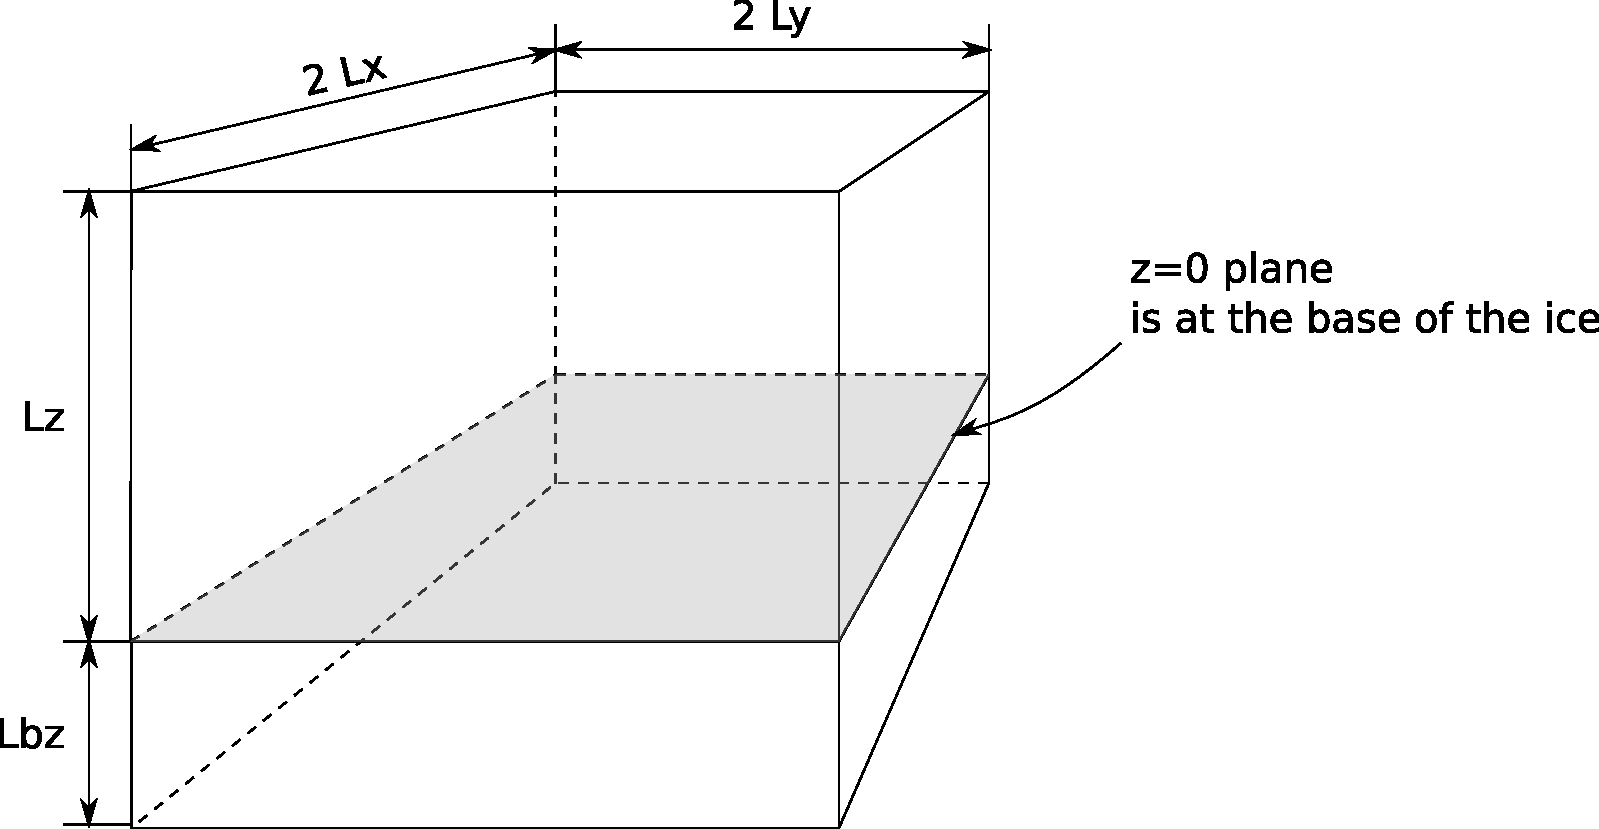
\includegraphics[width=4.0in,keepaspectratio=true]{rectilinearbox}
\caption{PISM's computational box.}
\label{fig:rectilinearbox}
\end{figure}


\subsection{Spatial grid}
\label{subsect:grid}
\optsection{Grid!space}

The PISM grid\index{PISM!grid} covering the computational box is equally spaced in horizontal ($x$ and $y$) directions.  Vertical spacing in the ice is quadratic by default (see below) but optionally a different spacing scheme can be chosen.  (Choose with options \txtopt{z_spacing}{[quadratic, equal]}.) The bedrock thermal layer model always uses equal vertical spacing.

The grid is described by four numbers, namely the number of grid points \texttt{Mx} in the $x$ direction, the number \texttt{My} in the $y$ direction, the number \texttt{Mz} in the $z$ direction within the ice, and the number \texttt{Mbz} in the $z$ direction within the bedrock thermal layer.  These are specified by options \intextoption{Mx}, \intextoption{My}, \intextoption{Mz}, and \intextoption{Mbz}, respectively. The defaults are 61, 61, 31, and 1, respectively.

Note that \texttt{Mx}, \texttt{My}, \texttt{Mz}, and \texttt{Mbz} all indicate the number of grid \emph{points}.  The numbers of grid \emph{spaces} are one less, thus 60, 60, 30, and 0 in the default case.  The lowest grid point in a column of ice, at $z=0$, coincides with the highest grid point in the bedrock, so \texttt{Mbz} must always be at least one and \texttt{Mbz}$>1$ is required to use the bedrock thermal model.  Note that this option is unrelated to the bed deformation model (glacial isostasy model); see option \texttt{-bed_def} (section \ref{subsect:beddef}) for that.

In the quadratic case, the spacing near the ice/bedrock interface is about four times finer than it would be with equal spacing for the same value of \texttt{Mz}, while the spacing near the top is correspondingly coarser. For a detailed description of the spacing of the grid, see the documentation on \texttt{IceGrid::compute_vertical_levels()} in the PISM class browser.

When a thermal bedrock layer is used, the distance \texttt{Lbz} is controlled by the \texttt{-Lbz} option.

If one initializes PISM from a saved model state using \t{-i} then the input model state controls all computational grid parameters.  For instance, the command

\begin{verbatim}
$  pismr -i foo.nc -y 100
\end{verbatim}

\noindent should work fine if \texttt{foo.nc} was a valid PISM model file.  The command

\begin{verbatim}
$  pismr -i foo.nc -Mz 201 -y 100
\end{verbatim}

\noindent will give a warning that ``\texttt{PISM WARNING: ignoring command-line option '-Mz'}'' because \texttt{-i} input files take precedence.

Otherwise, one is allowed to specify the grid when PISM is started.  In particular, the user should specify the grid when using \texttt{-boot_file} or when initializing a simplified-geometry experiment or a verification test, though defaults are generally present in the latter cases.  See sections \ref{sect:start} and \ref{sect:boot} for examples and explanation.


\subsection{Model time}
\label{sec:time}
\optsection{Grid!time}

The following command-line options control PISM time:

\begin{tabular}{lp{0.8\linewidth}}\\
\toprule
\textbf{Option} & \textbf{Meaning}\\
\midrule
\txtopt{y}{(years)} & Number of model years to run.\\
\txtopt{ys}{(years)} & Model year at which to start the run.  Also resets the model time, ignoring any time in the input file.\\
\txtopt{ye}{(years)} & Model year at which to end the run.\\
\bottomrule
\end{tabular}
\\[2em]
\noindent The default value for the end year is the start year (\texttt{-ys} or initialized model time from file) plus the default or given (\texttt{-y}) run length.  If both \texttt{-ys} and \texttt{-ye} are used then the run length is set to the difference.  Using all three of \texttt{-ys}, \texttt{-y} and \texttt{-ys} is not allowed.


\subsection{Diagnostic computations}
\label{sec:diagnostic-computations}

 As a diagnostic example, consider the second of these two runs:
\begin{verbatim}
pisms -y 6000 -o foo.nc
pismr -i foo.nc -y 0 -o bar.nc -o_size big
\end{verbatim}

\noindent The result of this zero-length, ``\texttt{-y 0}'', run is a NetCDF file \texttt{bar.nc} which contains the full three-dimensional velocity field in the scalar NetCDF variables \texttt{uvel}, \texttt{vvel}, and \texttt{wvel}, as well as many other variables.  The file \texttt{foo.nc} does not contain many of these fields because it was written with the default output size of \texttt{medium}.  The ``\texttt{-y 0}'' run has diagnostically ``filled-in'' the fields which PISM can model at a time step, but the model state has not evolved.

In fact, during such a run PISM performs one short time-step to compute ``rates of change'' of ice thickness, surface elevation and other fields, but the model state \emph{is reset} after this step, so re-starting from \texttt{foo.nc} above would give the same result as re-starting from \texttt{bar.nc}.

This diagnostic mode is most frequently associated to the modeling of ice shelves and ice streams.  Subsection \ref{sect:ross} describes using \texttt{pross} to model the Ross ice shelf \cite{MacAyealetal}.  Verification tests I and J, section \ref{sect:verif}, are diagnostic calculations using the SSA.

Note that the NetCDF model state saved by PISM at the end of an \emph{evolution} run does not, by default, contain the three-dimensional velocity field.  Instead, it contains just a bit more than the variables which are needed to restart the run.  One can  force PISM to save all the supported diagnostic quantities at the end of a time-stepping run using the option \texttt{-o_size big}.  Or one can go back and do a ``\texttt{-y 0}'' diagnostic run.


\subsection{Computing ice age} \label{subsect:age}
\optsection{Computing ice age}

By default, PISM does not compute the age of the ice\index{PISM!modeling the age of the ice} because it does not directly impact ice flow when using the default flow laws. It is very easy to turn on.  Just set \intextoption{age}.

  
\subsection{Flotation criterion and mask} \label{subsect:floatmask}  The most basic decision about ice dynamics made internally by PISM is whether to apply the ``flotation criterion'' to determine whether the ice is floating on the ocean or not.  In an evolution run this decision is made at each time step and the result is stored in the \t{mask}.

The possible values of the \t{mask}\index{mask} are given in Table \ref{tab:maskvals}.  The mask does not by itself determine ice dynamics.  For instance, when ice is floating (either value \texttt{MASK_FLOATING} or \texttt{MASK_FLOATING_AT_TIME_0}) the usual choice for ice dynamics is SSA, but the user can choose not to apply that model by not using either option \texttt{-ssa_floating_only} or \texttt{-ssa_sliding}.

\begin{table}[ht]
  \centering
  \caption{The PISM mask\index{mask}, in combination with user options, determines the dynamical model.}\label{tab:maskvals} 
  \small
  \begin{tabular}{p{0.25\linewidth}p{0.65\linewidth}}
    \toprule
    \textbf{Mask value} & \textbf{Meaning}\\\midrule
    1=\texttt{MASK_SHEET} & ice is grounded (and only the SIA is always applied) \\
    2=\texttt{MASK_DRAGGING_SHEET} & ice is grounded (and the SSA is applied if option \texttt{-ssa} is given) \\
    3=\texttt{MASK_FLOATING} & ice is floating (and the SSA is applied if option \texttt{-ssa} is given) \\
    7=\texttt{MASK_FLOATING_AT_TIME_0} & same as \texttt{MASK_FLOATING}, but the grid point was ice free ocean at initialization of the model by \texttt{-boot_file}; ice with this value will calve off if option \texttt{-ocean_kill} is given.
    \\\bottomrule
  \end{tabular}
  \normalsize
\end{table}

Assuming the geometry of the ice evolves (which can be turned off by option \texttt{-no_mass}), and assuming an ocean exists (which can be turned off by option \texttt{-dry}), then at each time step the mask changes by the flotation criterion.  Ice which becomes floating is marked as \texttt{MASK_FLOATING} while ice which becomes grounded is either marked as \texttt{MASK_SHEET} or \texttt{MASK_DRAGGING}.  The latter case occurs if the option \texttt{-ssa_sliding} is used, while otherwise all points are marked \texttt{MASK_SHEET}.


\subsection{Rheology}
\label{sec:rheology}
\optsection{Rheology}

In the polythermal (default) mode of PISM there is only one choice of the flow law: the Glen-Paterson-Budd-Lliboutry-Duval \cite{AschwandenBlatter,LliboutryDuval1985,PatersonBudd}. This law is the only one which we know of in the literature that parameterizes the (observed) softening of pressure-melting-temperature ice, as its liquid fraction increases.

Note that a ``flow law'' here means the function $F(\sigma,T,\omega,P,d)$ in the relation
	$$\dot \eps_{ij} = F(\sigma,T,\omega,P,d)\, \sigma_{ij}'$$
where $\dot \eps_{ij}$ is the strain rate tensor, $\sigma_{ij}'$ is the stress deviator tensor, $T$ is the ice temperature, $\omega$ is the liquid water fraction in the ice, $\sigma^2 = \frac{1}{2} \|\sigma_{ij}'\|_F$, so $\sigma$ is the second invariant of the stress deviator tensor, $P$ is the pressure, and $d$ is the grain size. For example, $F = A \sigma^{n-1}$ is the isothermal Glen law.. That is, we are addressing isotropic flow laws only.  In PISM one can choose the scalar function $F$ reasonably arbitrarily by modifying source code,\footnote{See source files \texttt{flowlaws.hh}, \texttt{flowlaws.cc} in \texttt{src/base/rheology/}.} or use the single polythermal law (above), or choose among a number of ``cold ice'' laws listed in table \ref{tab:flowlaw}.

Note that the inverse form of such a flow law in needed for ice shelves and ice streams:
	$$\sigma_{ij}' = 2 \nu(\dot\eps,T,\omega,P,d)\,\dot \eps_{ij} $$
Here $\nu(\dot \eps,T,\omega,P,d)$ is the effective viscosity.

The command-line options \intextoption{sia_e} and \intextoption{ssa_e} set flow enhancement factors for the SIA and SSA respectively. These options can be used with any flow law.  (The enhancement factor $e$ alters the SIA flow law to be ``$\dot \eps_{ij} = e\, F(\sigma,T,\omega,P,d)\, \sigma_{ij}'.$'')

The command-line option \intextoption{flow_law} control the flow law in the \texttt{-cold} mode.  Arguments to \texttt{-flow_law} are in table \ref{tab:flowlaw} below.

Flow law parameters such as ice softness can be changed using configuration parameters (see section \ref{sec:pism-defaults}) and the implementation of flow laws in the \emph{Source Code Browser}.

\begin{table}[ht]
\centering
\caption{\emph{For} \texttt{-cold} \emph{mode only:} Choosing the rheology using \t{-flow_law}.}\label{tab:flowlaw}\index{rheology}\index{flow law}
\small
\begin{tabular}{p{0.15\linewidth}p{0.2\linewidth}p{0.6\linewidth}}\toprule
\textbf{Type} & C++ Class & \textbf{Comments and Reference} \\ \midrule
\t{pb} &\texttt{ThermoGlenIce}  & Paterson-Budd law, the cold-mode default.  Fixed Glen exponent $n=3$.  There is a split ``Arrhenius'' term $A(T) = A \exp(-Q/RT^*)$ where \mbox{$A = 3.615 \times 10^{-13}\, \text{s}^{-1}\, \text{Pa}^{-3}$}, \mbox{$Q = 6.0 \times 10^4\, \text{J}\, \text{mol}^{-1}$} if $T^* < 263$ K and
 \mbox{$A = 1.733 \times 10^{3}\, \text{s}^{-1}\, \text{Pa}^{-3}$}, \mbox{$Q = 13.9 \times 10^4\, \text{J}\, \text{mol}^{-1}$} if $T^* > 263$ K and where $T^*$ is the pressure-adjusted temperature \cite{PatersonBudd}. \\
\t{arr} &  \texttt{ThermoGlenArrIce} & \emph{Cold} part of Paterson-Budd.  Regardless of temperature, the $A$ and $Q$ values for $T^*<263$ K in  the Paterson-Budd law apply.  This is the flow law used in the thermomechanically coupled exact solutions Tests \textbf{F} and \textbf{G} described in \cite{BBL,BB} and run by \texttt{pismv -test F} and \texttt{pismv -test G}. \\
\t{arrwarm} & \texttt{ThermoGlenArrIceWarm} & \emph{Warm} part of Paterson-Budd.  Regardless of temperature, the $A$ and $Q$ values for $T^*>263$ K in Paterson-Budd apply.\\
\t{hooke} & \texttt{HookeIce} & Hooke law.  Fixed Glen exponent $n=3$.  Here  \mbox{$A(T) = A \exp(-Q/(RT^*) + 3C (T_r - T^*)^\kappa)$;} values of  constants as in \cite{Hooke,PayneBaldwin}.\\
\t{gk} & \texttt{GoldsbyKohlstedtIce} & The  Goldsby-Kohlstedt flow law.  This law has a combination of exponents  from $n=1.8$ to $n=4$ \cite{GoldsbyKohlstedt}. It does not have a viscosity form and can only be used by the SIA stress balance. \\
\t{isothermal_glen} &  \texttt{IsothermalGlenIce} &The isothermal Glen flow law. \\
\bottomrule
\normalsize	
\end{tabular}
\end{table}

\subsection{Choosing the stress balance}  \label{subsect:ssacontrol}
\optsection{SSA as a sliding law}

The shallow shelf approximation (SSA)\index{SSA (shallow shelf approximation)} stress balance is used in PISM to describe the sliding of grounded ice and the formation of ice streams \cite{BBssasliding}, as well as being used as the only stress balance for floating ice.  For the SSA with ``plastic'' or ``Coulomb'' till locations of ice streams are determined as part of a free boundary problem identified by Schoof \cite{SchoofStream}.  We believe that this mathematical description of ice streams should be regarded as the best existing ``sliding law'' for the SIA \cite{BBssasliding}.\index{SIA (shallow ice approximation)!sliding laws}

Schoof's model \cite{SchoofStream} describes emergent ice streams within a larger ice sheet and ice shelf system.  It explains the existence of ice streams by a combination of the plastic failure of the till and the SSA approximation of the balance of momentum.  

In PISM the user gives the option \texttt{-ssa_sliding} to turn on the use of the plastic till SSA as a sliding law.  All grounded points are immediately marked as SSA (i.e.~as \texttt{DRAGGING}).  As explained in the next subsection, at these points a yield stress is computed from the amount of stored basal water and from a (generally) spatially-varying till strength, \texttt{tillphi} in an input or output file.  The amount of stored basal water is thermodynamically determined.

\begin{table}[ht]
\centering
\caption{The basic choice of stress balance.}\label{tab:stressbalchoice} 
\small
\begin{tabular}{p{0.25\linewidth}p{0.65\linewidth}}\toprule
\textbf{Option} & \textbf{Semantics}\\ \midrule
    (\emph{NO OPTION}) & Grounded ice flows by the non-sliding SIA.  (Floating ice essentially doesn't flow, so this model is not recommended for marine ice sheets.) \\
    \intextoption{ssa_floating_only} & Only floating ice uses SSA.  Grounded ice marked by mask value \texttt{SHEET} uses the (by default) nonsliding SIA. \\
\intextoption{ssa_sliding} & The recommended default sliding law, which gives the SIA+SSA hybrid stress balance.  Combines SSA-computed velocity, using pseudo-plastic till, with SIA-computed velocity according to the combination in \cite{BBssasliding}.  Floating ice uses SSA only. \\
\bottomrule\end{tabular}
\normalsize
\end{table}

%\intextoption{ice_reg_schoof_length} (1000 km) & Set the ``$L$'' in formula (4.1) in \cite{SchoofStream}.  To use the regularization described by Schoof, one must set \texttt{-ssa_eps 0.0} to turn off the other regularization mechanism, otherwise there is a double regularization (the default except in \texttt{ssa_testi}). \\
%\intextoption{ice_reg_schoof_vel} (1 m/a) & Set the \emph{first} ``$\eps$'' in formula (4.1) in \cite{SchoofStream}.  To deactivate Schoof's regularization, use \texttt{-ice_reg_schoof_vel 0}.  To use the regularization described by Schoof, one must set \texttt{-ssa_eps 0.0} to turn off the other regularization mechanism, otherwise there is a double regularization (the default except in \texttt{ssa_testi}).  Use \texttt{-plastic_reg} above to set the second ``$\eps$'' in formula (4.1) of \cite{SchoofStream}. \\

\begin{table}
  \centering
  \caption{Controlling the SSA stress balance in PISM}
 \begin{tabular}{p{0.2\linewidth}p{0.75\linewidth}}
   \label{tab:ssausage}\\\toprule
   \textbf{Option} & \textbf{Description}\\\midrule
\intextoption{ssa_maxi} (300) & This option sets the maximum allowed number of nonlinear iterations in solving the shallow shelf approximation.  One should usually use option \texttt{-ssa_rtol} to control convergence of the nonlinear iteration.\\
\intextoption{ssa_eps} (1e-15) & The numerical scheme for the shallow shelf approximation  \cite{WeisGreveHutter} computes an effective viscosity which which depends on velocity and temperature.  After that computation, this constant is added to the effective viscosity (to keep it bounded away from zero).  The units are kg $\text{m}^{-1}\,\text{s}^{-1}$.  By default, the regularization in equation (4.1) of \cite{SchoofStream} is also active, use \texttt{-ice_reg_schoof_vel 0} to deactivate Schoof's regularization. Turn off this lower bound mechanise by \texttt{-ssa_eps 0.0} to exclusively use the Schoof regularization mechanism; see \texttt{-ice_reg_schoof_vel} and \texttt{-ice_reg_schoof_length} below.  Note \texttt{-ssa_eps} is set to zero automatically when running \texttt{ssa_testi}. \\
\intextoption{ssa_rtol} (1.0e-4) & The numerical scheme for the shallow shelf approximation \cite{WeisGreveHutter} does a nonlinear iteration wherein velocities (and temperatures) are used to compute a vertically-averaged effective viscosity which is used to solve the equations for horizontal velocity.  Then the new velocities are used to recompute an effective viscosity, and so on.  This option sets the relative change tolerance for the effective viscosity.
In particular, the nonlinear part of the iteration requires that successive values $\nu^{(k)}$ of the vertically-averaged effective viscosity satisfy
	$\frac{\|(\nu^{(k)} - \nu^{(k-1)}) H\|_2}{\|\nu^{(k)} H\|_2} \le \text{ssa_rtol}$
in order to end the iteration with $\nu = \nu^{(k)}$.  See also \texttt{-ksp_rtol}, a PETSc option below, as one may want to require a high relative tolerance for the linear iteration as well.\\
\bottomrule
\end{tabular}
\end{table}


\subsection{Surface gradient method}
\label{subsect:gradient}
\optsection{Driving stress computation}

PISM computes surface gradients to determine the ``driving stress''
	$$(\tau_{d,x},\tau_{d,y}) = - \rho g H \grad h,$$
where $H$ is the ice thickness, and $h = H+b$ is the ice surface elevation.  The driving stress enters into both the SIA and SSA stress balances, but in the former the driving stress is needed on a staggered grid, while in the latter the driving stress is needed on the regular grid.

Surface gradients are computed by finite differences in several slightly-different ways.  There are options for choosing which method to use, but to the best of our knowledge there is no over-arching theoretical advice on the best, most robust mechanism.  There are three methods in PISM, chosen by option \intextoption{gradient}:

\noindent\texttt{-gradient mahaffy}\quad  This most ``standard'' way computes the surface slope onto the staggered grid for the SIA \cite{Mahaffy}.  It makes $O(\Delta x^2,\Delta y^2)$ errors.  For computations of driving stress on the regular grid, centered differencing is used instead.

\noindent\texttt{-gradient haseloff}\quad  This is the default method, but it only differs from the Mahaffy method at ice-margin locations.  It alters the formula for the slope in those cases where an adjacent ice-free bedrock surface elevation is above the ice elevation.  The scheme only differs from \texttt{mahaffy} at such unusual margin points.

\noindent\texttt{-gradient eta}\quad  In this method we first transform the thickness $H$ by $\eta = H^{(2n+2)/n}$ and then differentiate the sum of the thickness and the bed using centered differences:
	$$\grad h = \grad H + \grad b = \frac{n}{(2n+2)} \eta^{(-n-2)/(2n+2)} \nabla \eta + \nabla b.$$
Here $b$ is the bed elevation and $h$ is the surface elevation.  This transformation sometimes has the benefits that the surface values of the horizontal velocity and vertical velocity, and the driving stress, are better behaved near the margin.  See \cite{BLKCB,CDDSV} for technical explanation of this transformation and compare \cite{SaitoMargin}.  The actual finite difference schemes applied to compute the surface slope are similar to option \texttt{mahaffy}.


\subsection{Schoof's parameterization of bed roughness in the SIA} \label{subsect:bedsmooth} \index{Schoof's parameterization of bed roughness}
\optsection{Schoof's parameterization of bed roughness}

Christian Schoof's article \emph{The effect of basal topography on ice sheet dynamics} from 2003 \cite{Schoofbasaltopg2003} describes how to alter the SIA model to more-effectively reproduce ice flow in the vicinity of significant subglacial bedrock topgraphy.  This theory explains that one should use a smoothed (spatially-averaged) bed, but then lower the SIA diffusivity in a precise way in those regions where the significant topography was smoothed-away.  As a practical matter for PISM, this theory improves the SIA model's ability to handle bed roughness because it parameterizes the effects of "higher-order" stresses which act on the ice as it flows over bed topography.   But it also provides a double performance boost, because smoothed beds give longer time steps through the adaptive time-stepping mechanism, \emph{and} because the reduction of diffusivity, which is the parameterized effect of the local bed roughness, gives even longer time-steps.  For a technical description of PISM's implementation of this theory, see the \emph{Browser} page ``Using Schoof's (2003) parameterized bed roughness technique in PISM''.

There is one option which controls this mechanism: \intextoption{bed_smoother_range} gives the half-width of the square smoothing domain in meters.  If zero is given, \texttt{-bed_smoother_range 0} then the mechanism is turned off.  The mechanism is on by default using executable \texttt{pismr}, with the half-width set to 5 km (\texttt{-bed_smoother_range 5.0e3}), giving the recommended smoothing size of 10 km \cite{Schoofbasaltopg2003}.  This mechanism is turned off by default in executables \texttt{pisms} and \texttt{pismv}.

PISM writes fields \texttt{topgsmooth}, \texttt{schoofs_theta}, \texttt{thksmooth} from this mechanism.  (Regarding the last, the thickness is never smoothed, but the thickness relative to the smoothed bedrock elevation, i.e.~the difference between the unsmoothed surface elevation and the smoothed bedrock elevation, is used internally in the mechanism.)


\subsection{Earth deformation models} \label{subsect:beddef} \index{earth deformation} \index{PISM!earth deformation models, using}
\optsection{Earth deformation models}

The option \txtopt{bed_def}{[none, iso, lc]} turns on bed deformation models.

The first model \verb|-bed_def iso|, is instantaneous pointwise isostasy.  This model assumes that the bed at the starting time is in equilibrium with the load.  Then, as the ice geometry evolves, the bed elevation is equal to the starting bed elevation minus a multiple of the increase in ice thickness from the starting time: $b(t,x,y) = b(0,x,y) - f [H(t,x,y) - H(0,x,y)]$.  Here $f$ is the density of ice divided by the density of the mantle, so its value is determined by setting the values of \verb|lithosphere_density| and \verb|ice_density| in the configuration file; see subsection \ref{sec:pism-defaults}.  For an example and verification, see Test H in Verification section. 

The second model \verb|-bed_def lc| is much more effective.  It is based on papers by Lingle and Clark \cite{LingleClark}\index{People!Lingle, Craig} \index{People!Clark, J.} and Bueler and others \cite{BLKfastearth}.  It generalizes and improves the most widely-used earth deformation model in ice sheet modeling, the flat earth Elastic Lithosphere Relaxing Asthenosphere (ELRA) model \cite{Greve2001}.  It imposes  essentially no computational burden because the Fast Fourier Transform is used to solve the linear differential equation \cite{BLKfastearth}.  When using this model in PISM, the rate of bed movement (uplift) is stored in the PISM output file and then is used to initialize the next part of the run.  In fact, if gridded ``observed'' uplift data is available, for instance from a combination of actual point observations and/or paleo ice load modeling, and it that uplift field is put in a NetCDF variable with standard name \verb|tendency_of_bedrock_altitude| in the  \texttt{-boot_file} file, then this model will initialize so that it starts with the given uplift rate.

Minimal example runs to compare these models:
\begin{verbatim}
$ mpiexec -n 4 pisms -eisII A -y 8000 -o eisIIA_nobd.nc
$ mpiexec -n 4 pisms -eisII A -bed_def iso -y 8000 -o eisIIA_bdiso.nc
$ mpiexec -n 4 pisms -eisII A -bed_def lc -y 8000 -o eisIIA_bdlc.nc
\end{verbatim}
Compare the \texttt{topg}, \texttt{usurf}, and \texttt{dbdt} variables in the resulting output files.

Test H in section \ref{sect:verif} can be used to reproduce the comparison done in \cite{BLKfastearth}.

\subsection{Disabling PISM components}
\label{sec:turning-off}
\optsection{Disabling PISM components}

Major model components, unlike ``peripheral'' ones like bed deformation, do not need to be turned ``on'' explicitly.\footnote{It would be a hassle to ask for SIA computations every time you need them, for example.} However, in some cases it is useful to be able to disable particular components (during model spin-up, for example). Currently PISM has switches disabling the mass-continuity step (command-line option \intextoption{no_mass}), energy balance computation (option \intextoption{no_energy}) and polythermal energy balance computation: option \intextoption{cold} makes PISM use temperature instead of enthalpy in the energy balance code.

%%% Local Variables: 
%%% mode: latex
%%% TeX-master: "manual"
%%% End: 

% LocalWords:  intercomparison PDD polythermal Lliboutry Duval
